% 1.1.Download.tex
%	Last update: 2019/12/19 F.Kanehori
%\newpage
\subsection{ダウンロード}
\label{subsec:Download}

\noindent
\SprLib はGitHubで管理されており、
次のURLからダウンロードすることができます。
以下、ダウンロードするディレクトリを\SprTop{}として説明を進めます。

\CmndLine{%
	> chdir C:/Springhead\\
	> git clone --recurse-submodules\Cont\\
	\Hskip{100pt}https://github.com/sprphys/Springhead
}{fig/command-2-1-a.eps}{DownloadTree1}
\medskip

\noindent
デフォルトでpythonが利用できる環境であればサブモジュールbuildtoolは必要ありませんし、
外部パッケージboost, glew, glut, glui を別途インストールして使用するのであれば
サブモジュールdependencyは必要ありません。

\noindent
そのような場合には次のようにしてサブモジュールを選択してください。
\begin{narrow}[s]
	\Vskip{-.2\baselineskip}\thinrule{\linewidth}\\
	サブモジュールを導入するのに必要なディスク容量は、
	buildtoolが約31MB、dependencyが約550MBです。\\
	\Vskip{-\baselineskip}\thinrule{\linewidth}\\
\end{narrow}

\CmndLine{%
	> chdir C:/Springhead\\
	> git clone https://github.com/sprphys/Springhead\\
	> git submodule update --init --checkout buildtool\\
	> git submodule update --init --checkout dependency
}{fig/command-2-1-b.eps}{DownloadTree2}

\medskip
Wndows exploreならば右クリックでGUIが利用できます。
図1の右図でrecursiveにチェックを入れるとサブモジュールも一緒にダウンロードできます。
\begin{narrow}[15pt]
	\begin{figure}[h]
	\begin{center}
	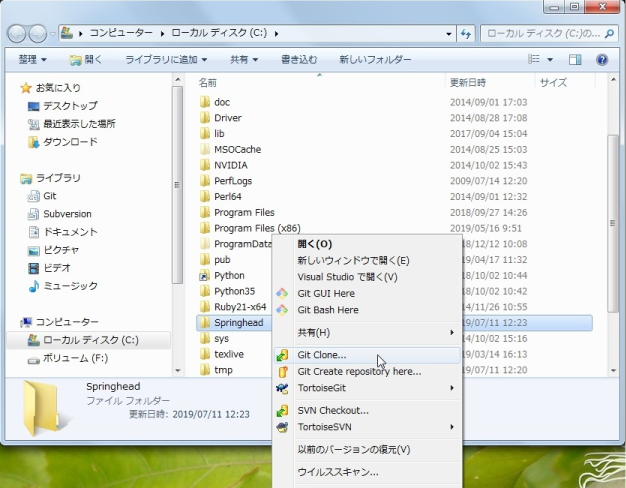
\includegraphics[width=0.5\textwidth]{fig/SpringheadClone1.eps}
	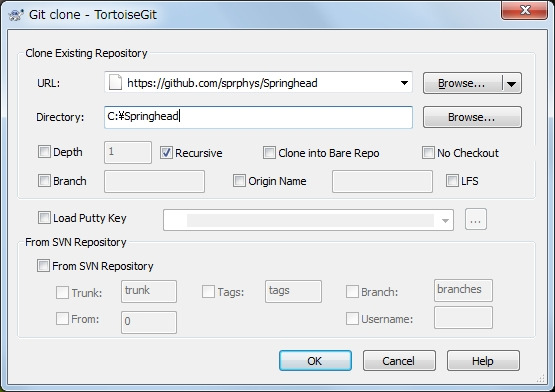
\includegraphics[width=0.4\textwidth]{fig/SpringheadClone2.eps}
	\end{center}
	\caption{Springheadダウンロード}
	\label{fig:SpringheadClone}
	\end{figure}
\end{narrow}

% end 1.1.Download.tex
